\documentclass[
   1pt,
   border=1pt,
   convert={density=100}
]{standalone}

\usepackage{pgf}
\usepackage{tikz}
\usetikzlibrary{arrows,automata}
\usepackage[latin1]{inputenc}

\renewcommand{\familydefault}{\ttdefault}

\begin{document}
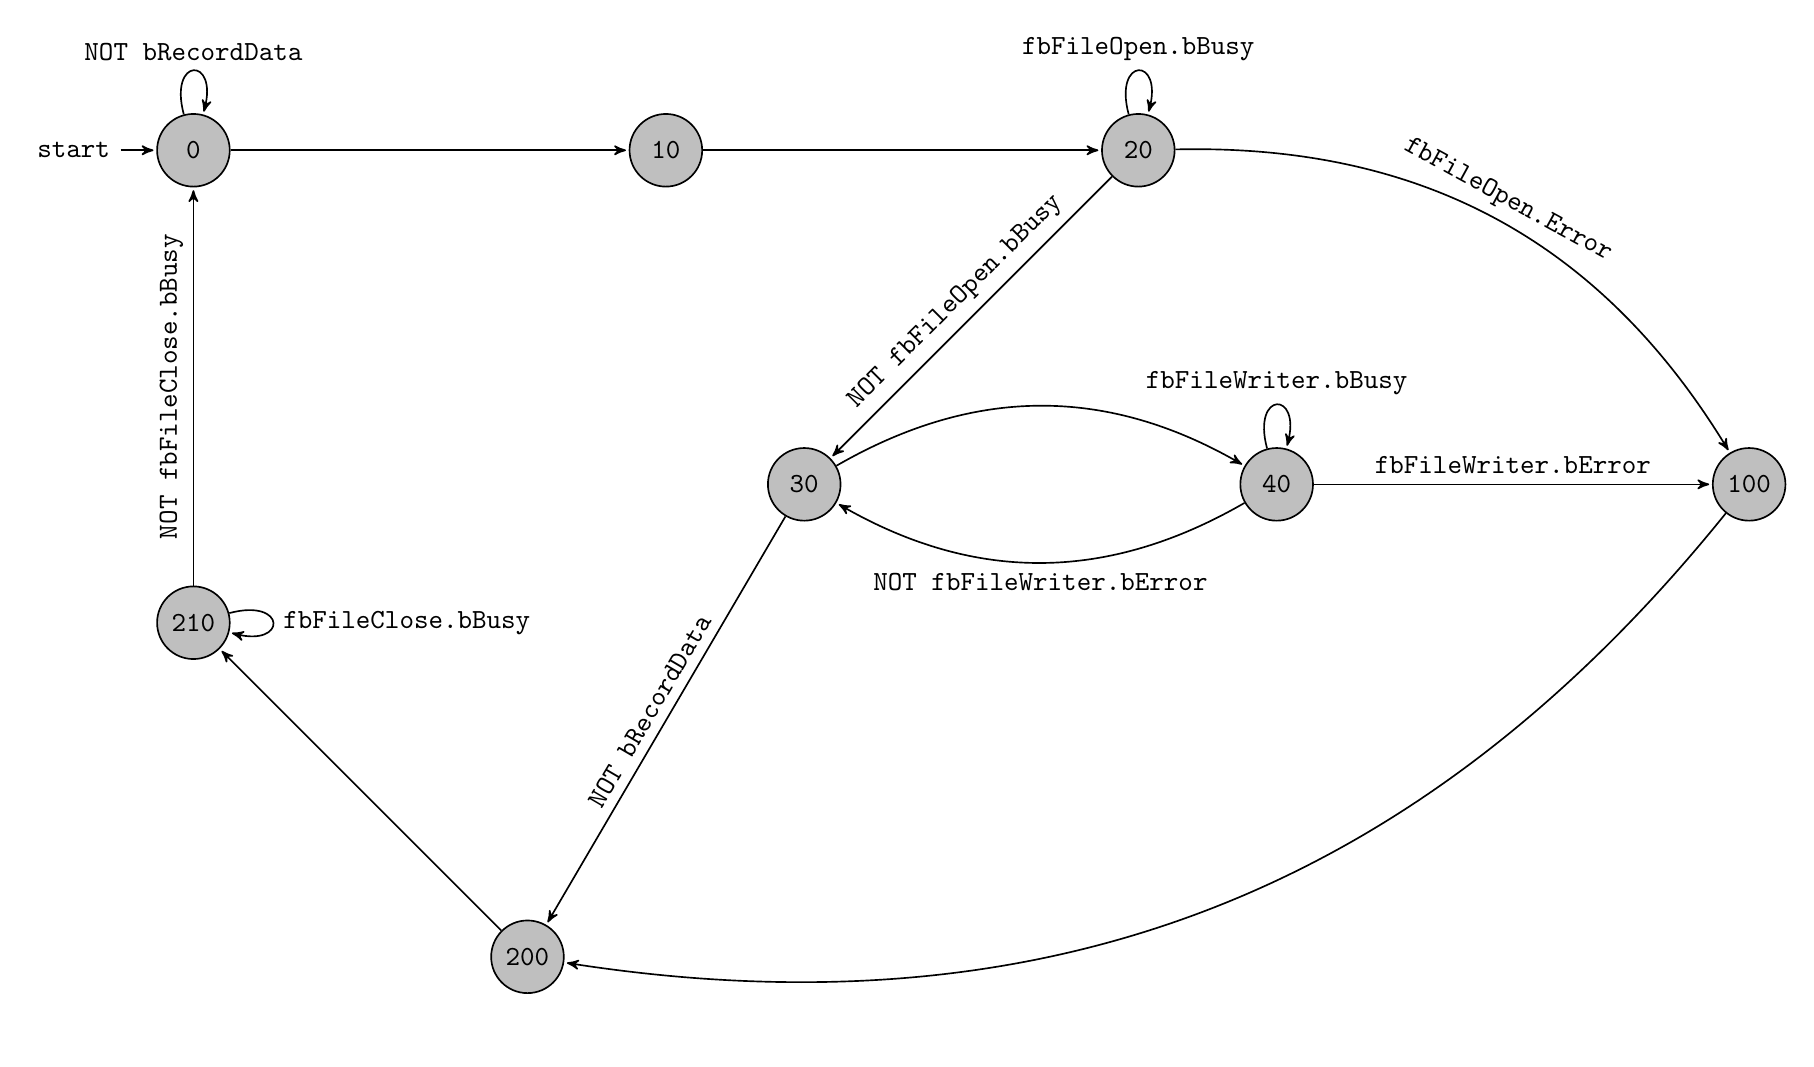
\begin{tikzpicture}[->,>=stealth',shorten >=1pt,auto,node distance=6cm,
                    semithick]
\tikzstyle{every state}=[fill=lightgray,draw=black,text=black]

\node[initial,state] 	(0) 	{0};
\node[state]		(10) 	[right of=0]			{10};
\node[state]		(20) 	[right of=10]			{20};
\node[state]		(30) 	[below left of=20]			{30};
\node[state]		(40) 	[right of=30]			{40};
\node[state]		(100) 	[right of=40]		{100};
\node[state]		(210) 	[below of=0]	{210};
\node[state]		(200) 	[below right of=210]	{200};


\path 	(0)	edge	[loop above]	node	{NOT bRecordData}	(0)
	(0)	edge			node	{}	(10)
	(10)	edge			node	{}	(20)
	(20)	edge	[loop above]	node	{fbFileOpen.bBusy}	(20)
	(20)	edge			node	[above, sloped]{NOT fbFileOpen.bBusy}	(30)
	(30)	edge	[bend left]	node	{}	(40)
	(40)	edge	[loop above]	node	{fbFileWriter.bBusy}	(40)
	(40)	edge	[bend left]	node	[below]{NOT fbFileWriter.bError}	(30)
	(30)	edge			node 	[above, sloped]{NOT bRecordData}	(200)
	(200)	edge			node 	{}	(210)
	(210)	edge			node 	[above, sloped]{NOT fbFileClose.bBusy}	(0)
	(210)	edge	[loop right]	node	{fbFileClose.bBusy}	(210)
	(20)	edge	[bend left]	node 	[above, sloped]{fbFileOpen.Error}	(100)
	(40)	edge			node 	{fbFileWriter.bError}	(100)
	(100)	edge	[bend left]	node	{}	(200);


\end{tikzpicture}

\end{document}